% ---------------------------------------------------------------------------
% TeX file of Revised LLNCS
% ---------------------------------------------------------------------------
% Extended LLNCS class, the original template is provided by:
% https://ctan.org/pkg/llncs
% The original example file is provided by:
% https://www.overleaf.com/latex/templates/springer-lecture-notes-in-computer-science/kzwwpvhwnvfj
%
% The template is extended by mostly used packages:
% ams*, tabular, graphicx, float, subfig, algorithm, hyperref, siunitx.
% ---------------------------------------------------------------------------
% Provided from the original template
% ---------------------------------------------------------------------------
% file typeinst.tex
%
% This is the LaTeX source for the instructions to authors using
% the LaTeX document class 'llncs.cls' for contributions to
% the Lecture Notes in Computer Sciences series.
% http://www.springer.com/lncs       Springer Heidelberg 2006/05/04
%
% It may be used as a template for your own input - copy it
% to a new file with a new name and use it as the basis
% for your article.
%
% NB: the document class 'llncs' has its own and detailed documentation, see
% ftp://ftp.springer.de/data/pubftp/pub/tex/latex/llncs/latex2e/llncsdoc.pdf
%

\documentclass[runningheads,a4paper,hyper]{llncsrev}

% Main Setup
\LLNCSRevSetup{
  % Configurations
  nohypercolor,  % hypercolor or nohypercolor
  ownerPass={}, userPass={},  % Only used in XeLaTeX
  % Short information mainly used in PDF strings.
  title={Chapter 1: Contribution Title},
  author={First Author, Second Author, and Third Author},
  institute={University of Houston}
}

% first the title is needed
\title{Chapter 1: Contribution Title\thanks{Supported by organization x.}}
% a short form should be given in case it is too long for the running head
\titlerunning{Contribution Title}

%
%\titlerunning{Abbreviated paper title}
% If the paper title is too long for the running head, you can set
% an abbreviated paper title here
%
\author{
  First Author\inst{1}\orcidID{0000-1111-2222-3333} \and
  Second Author\inst{1,2}\orcidID{1111-2222-3333-4444} \and
  Third Author\inst{2}\orcidID{2222--3333-4444-5555}
}
%
\authorrunning{F. Author et al.}
% First names are abbreviated in the running head.
% If there are more than two authors, 'et al.' is used.
%

% the affiliations are given next; don't give your e-mail address
% unless you accept that it will be published
\urldef{\mailsa}\path|{anna.kramer, leonie.kunz}@central.uh.com|
\urldef{\mailsb}\path|{christine.reiss, nicole.sator}@uni-heidelberg.de|
\institute{
  University of Houston, Houston, Texas, United States\\
  \mailsa \and
  ABC Institute, Rupert-Karls-University Heidelberg, Heidelberg, Germany\\
  \mailsb
}

%
% NB: a more complex sample for affiliations and the mapping to the
% corresponding authors can be found in the file "llncs.dem"
% (search for the string "\mainmatter" where a contribution starts).
% "llncs.dem" accompanies the document class "llncs.cls".
%
\toctitle{FWI with Low-frequency Extrapolation}
\tocauthor{F. Author et al.}

% Modification: the \keywords command is moved out from the abstract.
\keywords{first keyword, second keyword, third keyword}

% Configure the folders used for storing figures.
\graphicspath{{pics}}

\begin{document}
  
\mainmatter  % start of an individual contribution.

\maketitle  % Create the title.

\begin{abstract}
  The abstract should briefly summarize the contents of the paper in
  15--250 words.
\end{abstract}

\section{First Section}
\subsection{A Subsection Sample}
Please note that the first paragraph of a section or subsection is
not indented. The first paragraph that follows a table, figure,
equation etc. does not need an indent, either.

Subsequent paragraphs, however, are indented.

\subsubsection{Sample Heading (Third Level)} Only two levels of
headings should be numbered. Lower level headings remain unnumbered;
they are formatted as run-in headings.

\paragraph{Sample Heading (Fourth Level)}
The contribution should contain no more than four levels of
headings. Table~\ref{tab1} gives a summary of all heading levels.

\begin{table}
  \caption{Table captions should be placed above the
    tables.}\label{tab1}
  \begin{tabular}{|l|l|l|}
    \hline
    Heading level &  Example & Font size and style\\
    \hline
    Title (centered) &  {\Large\bfseries Lecture Notes} & 14 point, bold\\
    1st-level heading &  {\large\bfseries 1 Introduction} & 12 point, bold\\
    2nd-level heading & {\bfseries 2.1 Printing Area} & 10 point, bold\\
    3rd-level heading & {\bfseries Run-in Heading in Bold.} Text follows & 10 point, bold\\
    4th-level heading & {\itshape Lowest Level Heading.} Text follows & 10 point, italic\\
    \hline
  \end{tabular}
\end{table}


\noindent Displayed equations are centered and set on a separate
line.
\begin{equation}
  x + y = z
\end{equation}
Please try to avoid rasterized images for line-art diagrams and
schemas. Whenever possible, use vector graphics instead (see
Fig.~\ref{fig1}).

\begin{figure}
  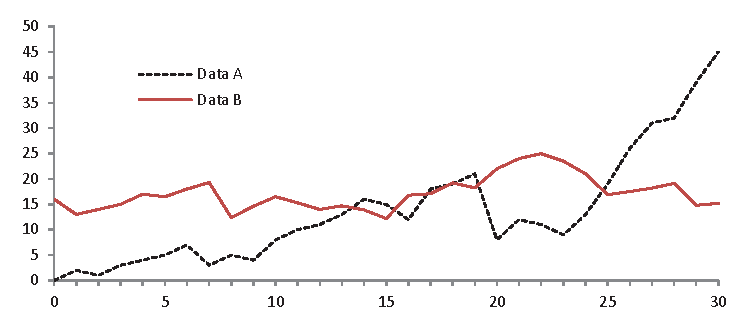
\includegraphics[width=\textwidth]{fig1.eps}
  \caption{A figure caption is always placed below the illustration.
    Please note that short captions are centered, while long ones are
    justified by the macro package automatically.} \label{fig1}
\end{figure}

\begin{theorem}
  This is a sample theorem. The run-in heading is set in bold, while
  the following text appears in italics. Definitions, lemmas,
  propositions, and corollaries are styled the same way.
\end{theorem}
%
% the environments 'definition', 'lemma', 'proposition', 'corollary',
% 'remark', and 'example' are defined in the LLNCS documentclass as well.
%
\begin{proof}
  Proofs, examples, and remarks have the initial word in italics,
  while the following text appears in normal font.
\end{proof}
For citations of references, we prefer the use of square brackets
and consecutive numbers. Citations using labels or the author/year
convention are also acceptable. The following bibliography provides
a sample reference list with entries for journal
articles~\cite{gridftp}, a chapter~\cite{peters2013chapter}, a
book~\cite{goodfellow2016deep}, proceedings without editors~\cite{apples1},
and a homepage~\cite{xilinxip}. Multiple citations are grouped
\cite{gridftp,peters2013chapter,goodfellow2016deep},
\cite{gridftp,goodfellow2016deep,apples1,xilinxip}.

\bibliographystyle{splncs04}        % Recommended by llncs (numbered citation format).
%\bibliographystyle{spbasic_unsrt}   % An alternative when using numbered citation format.
%\bibliographystyle{spbasic}         % Original format, not recommended (not sorted).
%\bibliographystyle{elsarticle-harv}  % When using author-year format.
\bibliography{bib/ref}

\end{document}
